\section{Problems}
\label{section:funcDecomProblems}
\graphicspath{ {./chapter05/FigSolutions} }

\begin{enumerate}
\def\labelenumi{\arabic{enumi}.}
\item
  Describe the differences between \emph{bottom-up} and \emph{top-down}
  design.

  \begin{onlysolution}
    \textbf{[R]}
    \itshape
    In a bottom-up design, the designer begins with basic components and 
    synthesizes them to create the overall system. However, the top-down 
    designer has a vision of the overall functionality of the final system 
    and partitions the problem into components, or subsystems. These components 
    work together to achieve the overall goal. In essences, bottom-up designers 
    are given parts and then they build the system, while top-down designers 
    envision the system and then build the parts.
  \end{onlysolution}
\item
  Develop a functional design for an audio graphic equalizer. A graphic
  equalizer decomposes an audio signal into component frequencies bands,
  allows the user to apply amplification to each individual band, and
  recombines the component signals. The design can employ either analog
  or digital processing. Be sure to clearly identify the design levels,
  functional requirements, and theory of operation for the different
  levels in the architecture.

The system must
\begin{itemize}
\item
  Accept an audio input signal source, with a source resistance of 1000Ω
  and a maximum input voltage of 1V peak-to-peak.
\item
  Have an adjustable volume control.
\item
  Deliver a maximum of 40W to an 8Ω speaker.
\item
  Have four frequency bands into which the audio is decomposed (you
  select the frequency ranges).
\item
  Operate from standard wall outlet power, 120V rms.
  \end{itemize}

  \begin{onlysolution}
    \textbf{[R]}
    \itshape
    \textbf{LEVEL 0}

    The Level 0 functionality for the audio graphic equalizer, shown below, 
    is fairly simple – the inputs are an audio signal, volume control, and 
    four frequency band knobs, and the output is a reconstructed audio signal.

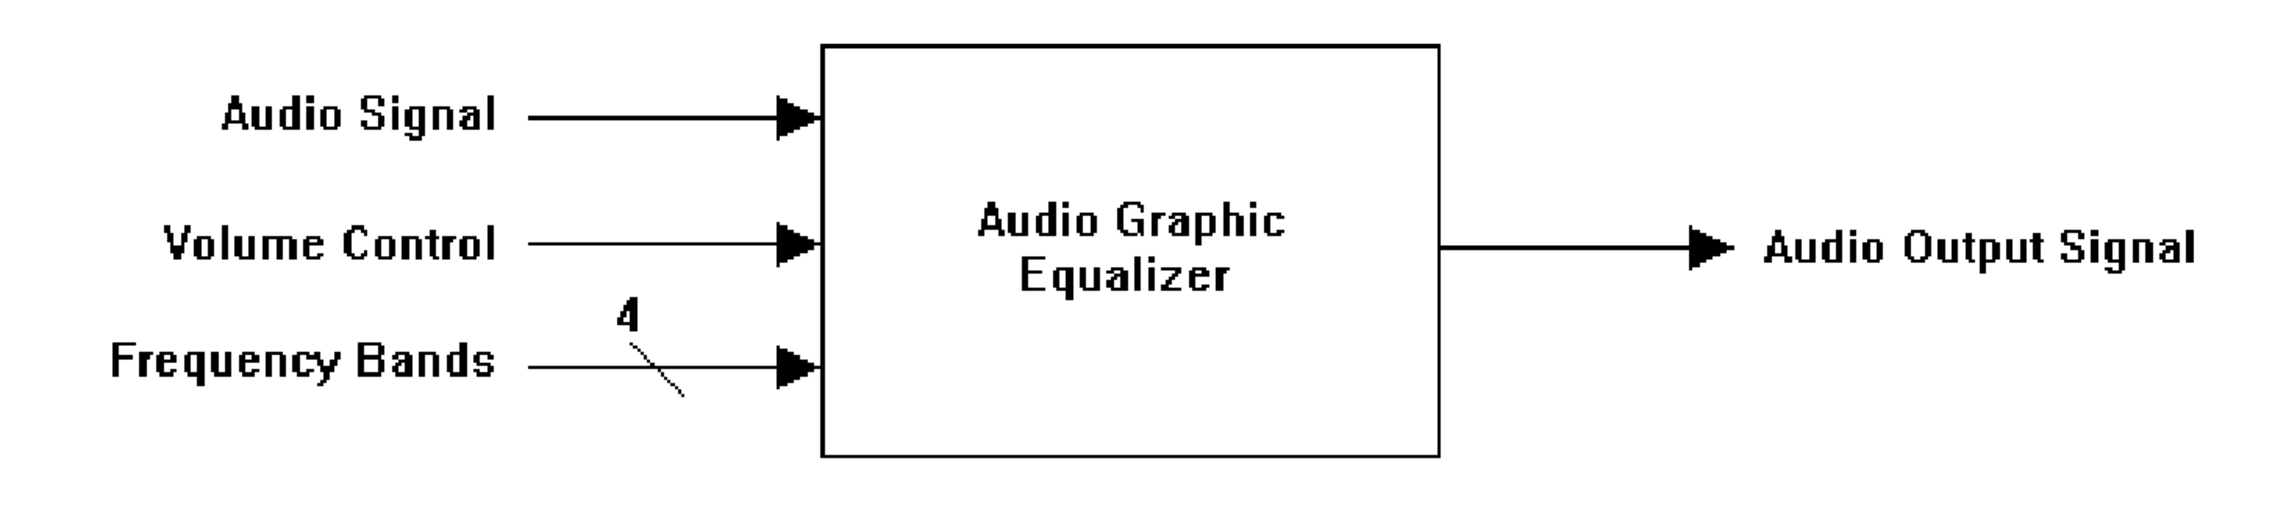
\includegraphics[width=0.8\textwidth]{image1}

\begin{tabular}{|l|m{10cm}|}
\hline
\emph{Module} & Audio Graphic Equalizer \\ \hline

\emph{Inputs} & 
\begin{itemize}
\item Audio input signal: 1Vpp , 1000$\Omega$
\item User volume control: variable control
\item Frequency band knobs: 4 bands (31Hz, 250Hz, 2KHz, 16KHz) , variable control.
\end{itemize} \\ \hline

\emph{Outputs} & 
\begin{itemize}
\item
  Audio output signal: \textul{?}V peak value.
\end{itemize}  \\ \hline

\emph{Functionality} & 
Reconstructs the input audio signal by amplifying and/or deamplifying each
of the 4 frequency bands to produce a 40W maximum output signal. The
volume amplification and frequency knobs should have variable user
control.
level. \\ \hline
\end{tabular}



Not all values can be known on the first pass through the design. However,
knowing the maximum power allows the maximum output voltage to be
computed as $V_{peak} = 8\Omega*40W = 17.9V$.

\textbf{Level 1}

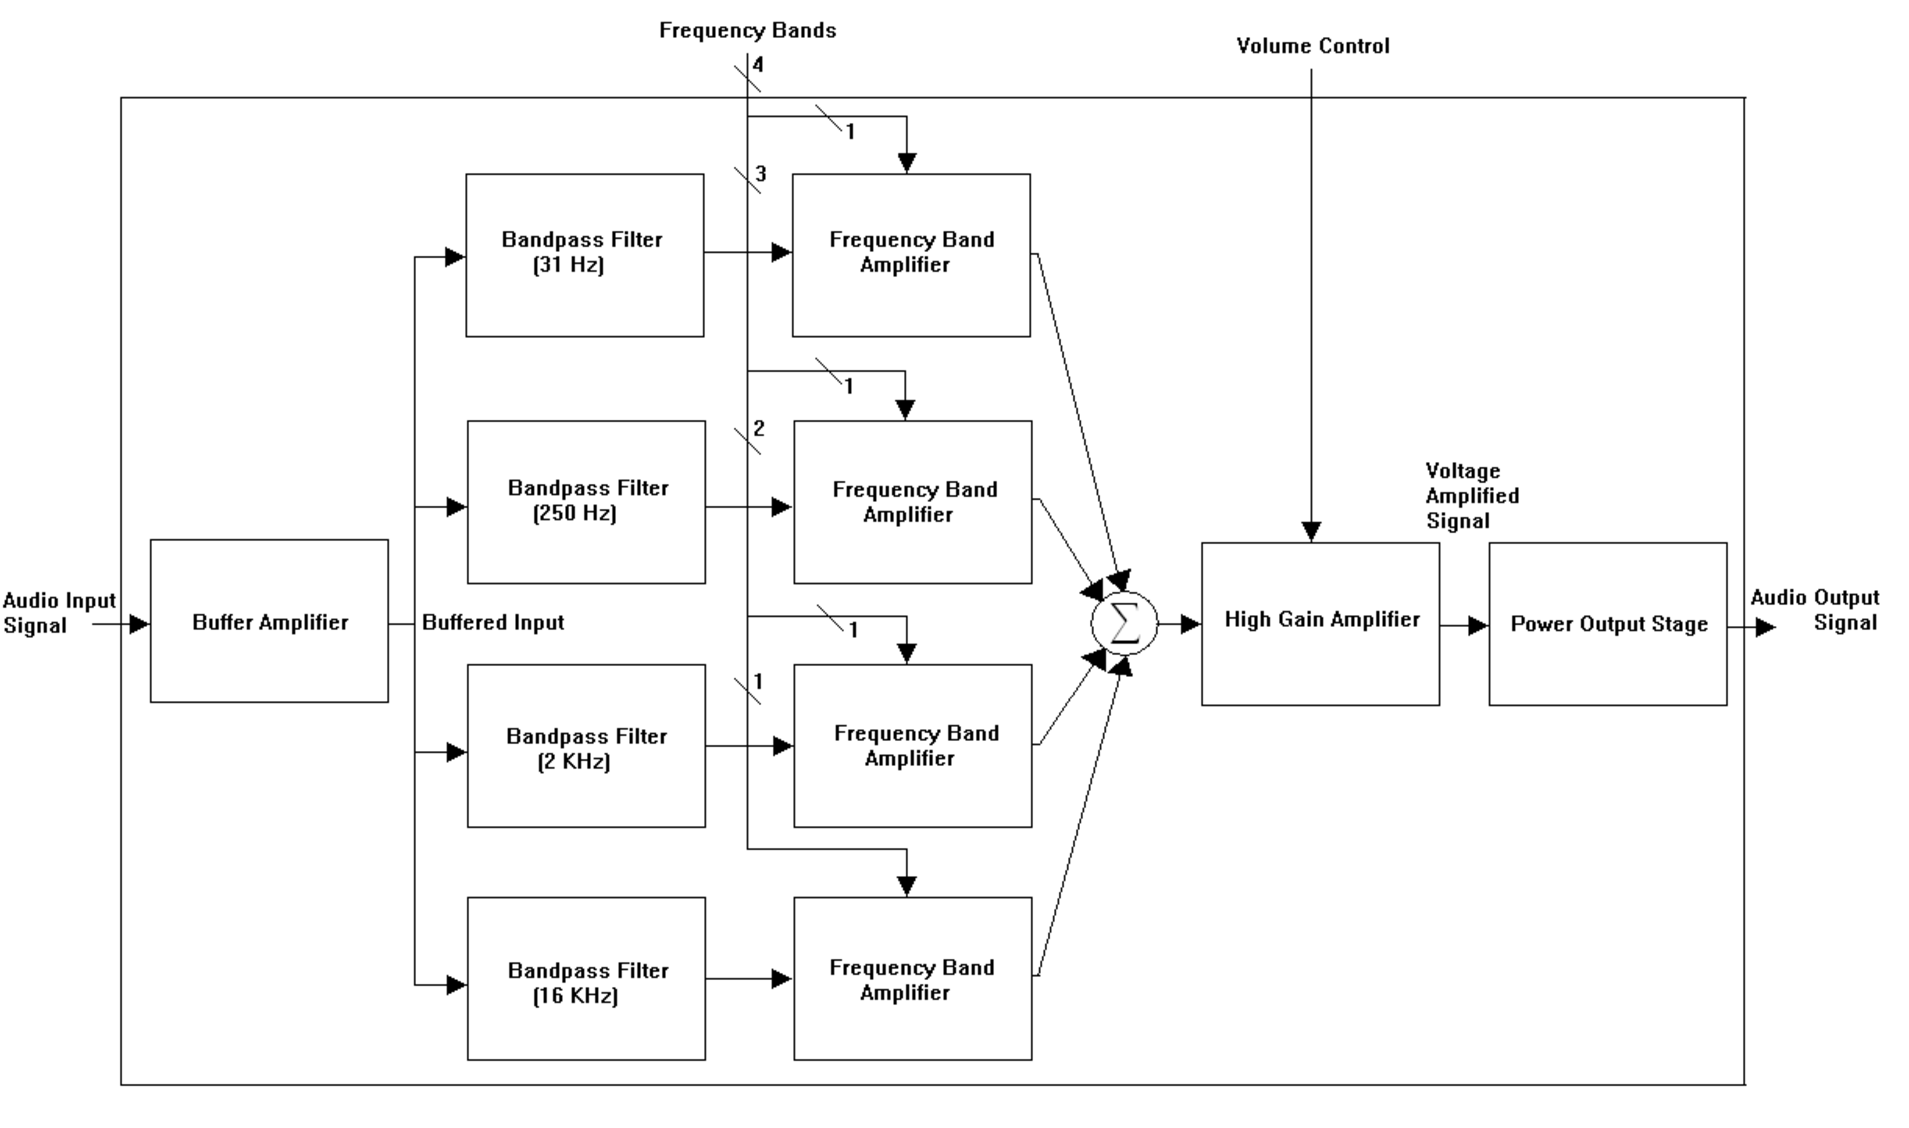
\includegraphics[width=0.9\textwidth]{image3}

There are several unknowns at this time, and that will be apparent as we
investigate the individual modules. The functional requirements for the Level 1
architecture are as detailed as possible, starting with the buffer amplifier.


\begin{tabular}{|l|m{10cm}|}
\hline
\emph{Module} &Buffer Amplifier\\ \hline

\emph{Inputs} & 
\begin{itemize}
\item Audio input signal: 1Vpp , 1000$\Omega$
\end{itemize} \\ \hline

\emph{Outputs} & 
\begin{itemize}
\item Audio output signal: 1Vpp , 1000$\Omega$
\end{itemize}  \\ \hline

\emph{Functionality} & 
Buffer the input signal and provide unity voltage gain. it should have an
input resistance of > 100k$\Omega$ and an output resistance < 100$\Omega$. \\ \hline
\end{tabular}

The input resistance is an educated guess, but is a realistically high value that will
minimize any voltage losses with the source resistance. The output resistance is
an educated guess, based on knowledge of what is achievable with the technology
(bottom-up knowledge). These resistance values are later refined and adjusted,
taking into account the input and output resistances for all stages.

\begin{tabular}{|l|m{10cm}|}
\hline
\emph{Module} & Bandpass Filters (0-31Hz, 31-250Hz, 250-2KHz, 2kHz-16KHz)\\ \hline

\emph{Inputs} & 
\begin{itemize}
\item Buffered input signal: 1Vpp , 1000$\Omega$
\end{itemize} \\ \hline

\emph{Outputs} & 
\begin{itemize}
\item Audio output signal: 17.9V peak value
\end{itemize}  \\ \hline

\emph{Functionality} & 
This filters out each of the desired frequency ranges so that they may be
adjusted independently. It should have an input resistance of > 1k$\Omega$ 
and an output resistance < 100$\Omega$. \\ \hline
\end{tabular}



\begin{tabular}{|l|m{10cm}|}
\hline
\emph{Module} & Frequency Band Amplifiers\\ \hline
\emph{Inputs} & 
\begin{itemize}
\item Filtered audio signals: 1Vpp , 1000$\Omega$
\item Frequency band knobs: 4 bands (31Hz, 250Hz, 2KHz, 16KHz) , variable control.
\end{itemize} \\ \hline
\emph{Outputs} & 
\begin{itemize}
\item Audio output signal: 17.9V peak value
\end{itemize}  \\ \hline
\emph{Functionality} & 
Functionality Provide an adjustable voltage gain, between 1 and 35, for each of the 4
frequency bands, respectively. It should have an input resistance of > 10k$\Omega$ 
and an output resistance < 100$\Omega$. \\ \hline
\end{tabular}


\begin{tabular}{|l|m{10cm}|}
\hline
\emph{Module} & Signal Summation\\ \hline
\emph{Inputs} & 
\begin{itemize}
\item  Audio input signals (31Hz, 250Hz, 2KHz, 16KHz): 1Vpp , 1000$\Omega$
\end{itemize} \\ \hline
\emph{Outputs} &  
\begin{itemize}
\item Audio output signal: 17.9V peak value
\end{itemize}  \\ \hline
\emph{Functionality} & 
Functionality This recombines each of the 4 frequencies that have be independently
adjusted into one complete signal.  It should have an input resistance of > 1k$\Omega$ 
and an output resistance < 100$\Omega$. \\ \hline
\end{tabular}


\begin{tabular}{|l|m{10cm}|}
\hline
\emph{Module} & High Gain Amplifier\\ \hline
\emph{Inputs} & 
\begin{itemize}
\item - Audio input signal: 1Vpp , 1000$\Omega$
\item User volume control: variable control
\end{itemize} \\ \hline
\emph{Outputs} &  
\begin{itemize}
\item Audio output signal: 17.9V peak value
\end{itemize}  \\ \hline
\emph{Functionality} & 
 It should have an input resistance of > 10k$\Omega$ 
and an output resistance < 100$\Omega$. \\ \hline
\end{tabular}

\begin{tabular}{|l|m{10cm}|}
\hline
\emph{Module} & Power Output Stage\\ \hline
\emph{Inputs} & 
\begin{itemize}
\item - Audio input signal: : 17.9V peak
\end{itemize} \\ \hline
\emph{Outputs} &  
\begin{itemize}
\item Audio output signal: 17.9V peak at up to \textul{???}A.
\end{itemize}  \\ \hline
\emph{Functionality} & 
Functionality Provide unity voltage gain with output current as required by a resistive load
of up to \textul{???}A.  It should have an input resistance of > 1k$\Omega$ 
and an output resistance < 100$\Omega$. \\ \hline
\end{tabular}



Note: there are other architectures that can work here as well. For example, the high
gain amplifier and power output stage can be combined into a single amplifier. In
addition, the filter and associated amplifiers might also be combined together,
depending upon the filter topology used.

  \end{onlysolution}
  
\item
  Develop a functional design for a system that measures and displays
  the speed of a bicycle. Be sure to clearly identify the design
  levels, functional requirements, and theory of operation for each
  level.\\
  The system must

\begin{itemize}
\item
  Measure instantaneous velocities between zero and 75 miles per hour
  with an accuracy of 1\% of full scale.
\item
  Display the velocity digitally and include one digit beyond the
  decimal point.
\item
  Operate with bicycle tires that have 19, 24, 26, and 27 inch
  diameters.
\end{itemize}

\begin{onlysolution}
  \textbf{[R]}
  \itshape
  \textbf{LEVEL 0}

  The overall goal is to convert a sensed speed to a digital speed reading 
  (i.e. speedometer).

%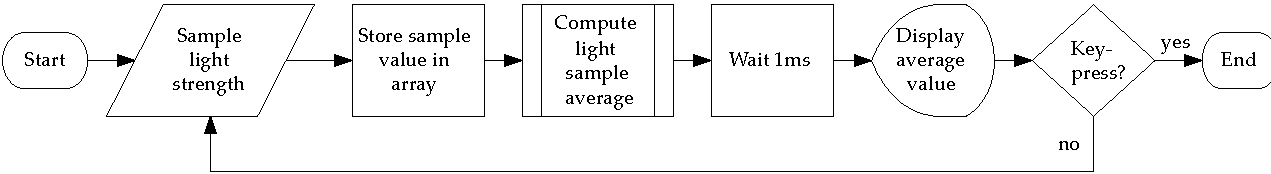
\includegraphics[width=0.8\textwidth]{image4}

\end{onlysolution}

  \item
    Draw a structure chart for the following C++ program:
\begin{verbatim}
void IncBy5(int \&a, int \&b);
int Multiply(int a, int b);
void Print(int a, int b);

main() {
    int x=y=z=0;
    IncBy5(x,y);
    z=Mult(x,y);
    Print(x,z);
}

void IncBy5(int \&a, int \&b) {
    a+=5;
    b+=5;
    Print(a,b);
}

int Multiply(int a, int b) {
    return (a*b);
}

void Print(int a, int b) {
    cout  << a << ``, `` << b;
}
\end{verbatim}

\begin{onlysolution}
  \textbf{[A]}
  \itshape
  ** add figure **
  \begin{center}
    \textbf{Structural Chart of C++ Program}
  \end{center}
\end{onlysolution}

\item
  Develop a functional design for software that meets the following
  requirements. \\
The system must

\begin{itemize}
\item
  Read an array of floating point numbers from an ASCII file on disk.
\item
  Compute the average, median, and standard deviation of the numbers.
\item
  Store the average, median, and standard deviation values on disk.
\end{itemize}

The design should have multiple modules and include the following
elements: (a) a structure chart, and (b) a functional description of
each module.



\item
  Describe in your own words what is meant by coupling in design.
  Describe the advantages of both loosely and tightly coupled designs.

  \begin{onlysolution}
    \textbf{[R]}
    \itshape
    Coupling describes a particular individual module’s dependence upon 
    the interconnectivity of various modules for proper functionality. 
    A module can be loosely coupled or tightly coupled. The advantages 
    of these are as follows:

    \textbf{Loosley Coupled}
    (+) The maximum degree of impact one module can have is limited 
    (+) May allow for continued functionality upon module failures
    (+) Maximizes the cohesion of a design
    (+) Allows for independent testing of modules

    \textbf{Tightly Coupled}
    (+) Better performance (i.e. software)
    (+) Quicker solutions (not necessarily better)

    It should be noted that the number of advantages of a loosely coupled 
    design usually outweigh that of a tightly coupled design.
  \end{onlysolution}

\item
  \textbf{Project Application.} Develop a functional design for your
  project. Follow the presentation guidelines in Section 5.9 for
  communicating the results of the design.

  \begin{onlysolution}
    \textbf{[R]}
    \itshape
    \emph{Note:} this is a major deliverable that is due for the project. 
    It is also tied closely in with Chapter 6 which also provides modern 
    design techniques. The information that we use in our assignment is 
    below.
  \end{onlysolution}

\end{enumerate}

